\section{FIXED WING UAV CONTROL}

\begin{yellowbox}{\textbf{NOMENCLATURE}}
    \begin{tabularx}{\columnwidth}{ll}
        $\delta_T\in[0,1]$ & Throttle control input (normalized)\\
        \addlinespace[2pt]
        $\delta_E\in[-1,1]$ & Elevator control input (normalized)\\
        \addlinespace[2pt]
        $\delta_A\in[-1,1]$ & Aileron control input (normalized)\\
        \addlinespace[2pt]
        $\delta_R\in[-1,1]$ & Rudder control input (normalized)
    \end{tabularx}
\end{yellowbox}

\begin{whitebox}{\textbf{REMARKS ON AIRCRAFT CONTROL}}
    \begin{itemize}
        \item Inherently nonlinear (especially longitudinal axis)
        \item Low control authority
        \item Actuator saturation
        \item Double integrator characteristics
        \item Underactuated MIMO system (4 inputs, 6 outputs/DOFs)
    \end{itemize}
\end{whitebox}

\begin{whitebox}{\textbf{CONTROL TECHNIQUES}}
    \begin{itemize}
        \item Cascaded PID loops
        \item Optimal control (LQR)
        \item Robust control ($H_\infty$, $H_2$ loop-sharing)
        \item Adaptive control
        \item Linear/nonlinear model predictive control
        \item (Nonlinear) dynamic inversion
    \end{itemize}
\end{whitebox}

\begin{whitebox}{\textbf{THE PLANT}}
    \begin{itemize}
        \item Control inputs $\delta_T,\delta_E,\delta_A,\delta_R$
        \begin{itemize}
            \item Positive deflections cause positive moments
            \item Ailerons may have differential (e.g. more "up" for same "down") to combat adverse yawing
        \end{itemize}
        \item States
        \begin{itemize}
            \item Body velocities $(u,v,w)$ estimated using Pitot-static tube ($V$), airflow vanes/multi-hole probe ($\beta,\alpha$) and GNSS ($_\mathcal{I}\bm{v}$)
            \item Body rates $(p,q,r)$ estimated using IMU gyroscope
            \item Euler angles $\phi,\theta,\psi$ estimated using IMU accelerometer ($_\mathcal{B}\bm{a}$) and magnetometer ($\psi$)
            \item Inertial position $r_N,r_E,r_D$ estimated using GNSS
        \end{itemize}
    \end{itemize}
\end{whitebox}

\begin{whitebox}{\textbf{PLANT LINEARIZATION}}
    \begin{itemize}
        \item Longitudinal plant
        \resizebox{0.8\linewidth}{!}{
            \includegraphics[
            page={79},
            trim = {1.5cm, 11.5cm, 12.8cm, 4.5cm}, % left, bottom, right, top
            clip
            ]{media/22HS_Lec11_Fixed_Wing_Dynamics_Compressed.pdf}
        }
        \item Lateral plant
        \resizebox{0.8\linewidth}{!}{
            \includegraphics[
            page={79},
            trim = {13.6cm, 11.5cm, 2.0cm, 4.5cm}, % left, bottom, right, top
            clip
            ]{media/22HS_Lec11_Fixed_Wing_Dynamics_Compressed.pdf}
        }
    \end{itemize}
\end{whitebox}

\begin{whitebox}{\textbf{CASCADED CONTROL LOOPS}}
    \begin{itemize}
        \item Control (low level part)
        \begin{itemize}
            \item Goal: Stabilize attitude
            \item Dynamics (actuator control inputs to states) challenging to globally identify in a nonlinear, high-fidelity form (thus linearizations common)
        \end{itemize}
        \item Guidance (high level part)
        \begin{itemize}
            \item Goals:
            \begin{itemize}
                \item Follow a reference trajectory (position control)
                \item Reject constant low-frequency disturbances e.g. constant wind
            \end{itemize}
            \item Dynamics typically only consist of kinematics (thus no system identification needed)
        \end{itemize}
    \end{itemize}
    \begin{center}
        \resizebox{0.7\linewidth}{!}{
            \includegraphics[
            page={73},
            trim = {15.0cm, 13.5cm, 1.5cm, 1.8cm}, % left, bottom, right, top
            clip
            ]{media/22HS_Lec11_Fixed_Wing_Dynamics_Compressed.pdf}
        }      
    \end{center}

\end{whitebox}

\begin{whitebox}{\textbf{SIMPLE CASCADED CONTROL}}
    \resizebox{1.0\linewidth}{!}{
        \includegraphics[
        trim = {3.0cm, 3.5cm, 2.2cm, 5.0cm}, % left, bottom, right, top
        clip
        ]{media/Simple_Cascaded_UAV_Control.pdf}
    }
    \begin{itemize}
        \item Need integrator wind-up protection
        \item Dynamic pressure scaling (scale actuator output inversely with airspeed i.e. $\sfrac{1}{V^2}$)
        \item Bandwidth (rate) of inner (low-level) loop should be sufficiently higher than outer (guidance) loop
    \end{itemize}
\end{whitebox}

\begin{whitebox}{\textbf{STATIONARY LEVEL COORDINATED TURN}}
    \begin{itemize}
        \item Stationarity: $_\mathcal{B}\dot{\bm{v}}_a=\bm{0}, _\mathcal{B}\Dot{\omega}=\bm{0}$
        \item Turning: $\phi=\mathrm{const.}\neq 0$
        \item Level: $\alpha=\theta\implies\gamma=0\implies h=\mathrm{const.}$
        \item Coordinated: $SF=0$ i.e. no sideslip $\beta=0\implies\xi=\psi$ (centripetal force only from lift component)
        \item Force balances in front view ($\perp\bm{v}_a$)
        \begin{align*}
            &L\cos\phi=mg\quad\\
            &\frac{mV^2}{R}=L\sin\phi+T\underbrace{\sin\epsilon_T}_{\approx 0}\sin\phi
        \end{align*}
        \item Minimum speed $V_{\min}\propto\sqrt{\sfrac{1}{\cos\phi}}$
        \item Heading/yaw rate $\Dot{\xi}=\Dot{\psi}=\sfrac{V}{R}=\frac{g\tan\phi}{V}$
        \item Additionally assume $D=T$ (thrust acts along drag axis)
    \end{itemize}
    \begin{center}
        \resizebox{0.7\linewidth}{!}{
            \includegraphics[
            page={64},
            trim = {16.0cm, 8.0cm, 0.0cm, 4.5cm}, % left, bottom, right, top
            clip
            ]{media/22HS_Lec11_Fixed_Wing_Dynamics_Compressed.pdf}
        }      
    \end{center}
\end{whitebox}

\begin{whitebox}{\textbf{$\mathcal{L}_1$ GUIDANCE}}
    \begin{itemize}
        \item Lateral-directional path following guidance (with stationary level coordinated turns)
        \begin{center}
            \resizebox{0.8\linewidth}{!}{
                \includegraphics[
                page={70},
                trim = {0.0cm, 3.0cm, 12.5cm, 6.5cm}, % left, bottom, right, top
                clip
                ]{media/22HS_Lec11_Fixed_Wing_Dynamics_Compressed.pdf}
            }     
        \end{center}
        \begin{itemize}
            \item Lookahead vector of length $L_1$
            \item Error angle $\eta$
            \item Roll reference $\phi_\mathrm{ref}$
            \begin{align*}
                &\sin\eta=\frac{L_1}{2R}\implies R=\frac{L_1}{2\sin\eta}\\
                &a_{s_\mathrm{cmd}}=\frac{V^2}{R}=\frac{2V^2\sin\eta}{L_1}\implies\Dot{\xi}_\mathrm{ref}=\frac{a_{s_\mathrm{cmd}}}{V}\\
                &\Dot{\xi}_\mathrm{ref}=\frac{g\tan\phi_\mathrm{ref}}{V}\implies\phi_\mathrm{ref}=\arctan\left(\frac{a_{s_\mathrm{cmd}}}{g}\right)
            \end{align*}
        \end{itemize}
    \end{itemize}
\end{whitebox}


\begin{whitebox}{\textbf{TOTAL ENERGY CONTROL SYSTEM (TECS)}}
    \begin{itemize}
        \item Control altitude and airspeed
        \begin{center}
            \resizebox{0.7\linewidth}{!}{
                \includegraphics[
                page={71},
                trim = {0.5cm, 3.0cm, 14.5cm, 9.0cm}, % left, bottom, right, top
                clip
                ]{media/22HS_Lec11_Fixed_Wing_Dynamics_Compressed.pdf}
            }      
        \end{center}
        \begin{itemize}
            \item Total energy $E$ (rate $\Dot{E}$)
                \begin{align*}
                    &E=E_K+E_P=\frac{1}{2}mV^2+mgH\\
                    &\frac{\Dot{E}}{mg}=\frac{V\Dot{V}}{g}+\Dot{H}
                \end{align*}
            \item Total energy $E_\mathrm{spec}$ (rate $\Dot{E}_\mathrm{spec}$)
                \begin{align*}
                    \Dot{E}_\mathrm{spec}=\frac{\Dot{E}}{mgV}=\frac{\Dot{V}}{g}+\frac{\Dot{H}}{V}=\frac{\Dot{V}}{g}+\sin\gamma\approx\frac{\Dot{V}}{g}+\gamma
                \end{align*}
            \item Energy distribution $E_\mathrm{dist}$ (rate $\Dot{E}_\mathrm{dist}$)
                \begin{align*}
                    \Dot{E}_\mathrm{dist}=\gamma-\frac{\Dot{V}}{g}
                \end{align*}
        \end{itemize}
        \resizebox{1.0\linewidth}{!}{
            \includegraphics[
            page={72},
            trim = {0.5cm, 2.0cm, 1.0cm, 6.0cm}, % left, bottom, right, top
            clip
            ]{media/22HS_Lec11_Fixed_Wing_Dynamics_Compressed.pdf}
        }
    \end{itemize}
\end{whitebox}